\ifmostrarGabarito
\begin{minted}{python}
import numpy as np
import matplotlib.pyplot as plt

def plotar_perfil_termoclina(
    tempos: np.ndarray,
    temperatura: np.ndarray,
    temp_critica: float,
    caminho_saida: str = "perfil_termoclina.pdf"
) -> bool:
    """
    Gera grafico orientado a objetos com curva termica, limiar critico e area sombreada.
    """
    fig, ax = plt.subplots(figsize=(10, 5))
    
    # 1. Plot da serie temporal continua com marcadores discretos
    ax.plot(
        tempos, temperatura,
        color="navy", linewidth=2.0, marker="o", markersize=4,
        label="Temperatura Medida (C)"
    )
    
    # 2. Linha tracejada horizontal de limite operacional
    ax.axhline(
        y=temp_critica, color="crimson", linestyle="--", linewidth=1.5,
        label=f"Limite Critico ({temp_critica:.1f}C)"
    )
    
    # 3. Area sombreada de alerta onde a temperatura excede o teto
    ax.fill_between(
        tempos, temperatura, temp_critica,
        where=(temperatura > temp_critica),
        color="crimson", alpha=0.25, label="Zona de Alerta Termico"
    )
    
    # 4. Customizacao textual e ambiental da figura
    ax.set_title("Monitoramento Termico do Meio de Propagacao Acustica", fontsize=13, fontweight="bold")
    ax.set_xlabel("Tempo de Operacao (min)", fontsize=11)
    ax.set_ylabel("Temperatura da Agua (C)", fontsize=11)
    ax.grid(True, linestyle=":", alpha=0.6)
    ax.legend(loc="upper right")
    
    # 5. Salvamento confinado e liberacao de memoria
    fig.savefig(caminho_saida, dpi=150, bbox_inches="tight")
    plt.close(fig)
    return True
\end{minted}

\textbf{Explicação:}
A solução adota o paradigma recomendado no Matplotlib (\texttt{fig, ax}):
\begin{itemize}[leftmargin=*]
    \item \texttt{ax.axhline}: Insere linhas de demarcação constante no eixo cartesiano.
    \item \texttt{ax.fill\_between(..., where=...)}: Destaca visualmente condições de anomalia ou risco sem exigir cálculo manual de polígonos.
    \item \texttt{plt.close(fig)}: Prática mandatória em ambientes de produção e servidores para prevenir vazamento de memória (\emph{memory leaks}).
\end{itemize}

\vspace{0.2cm}
\begin{center}
    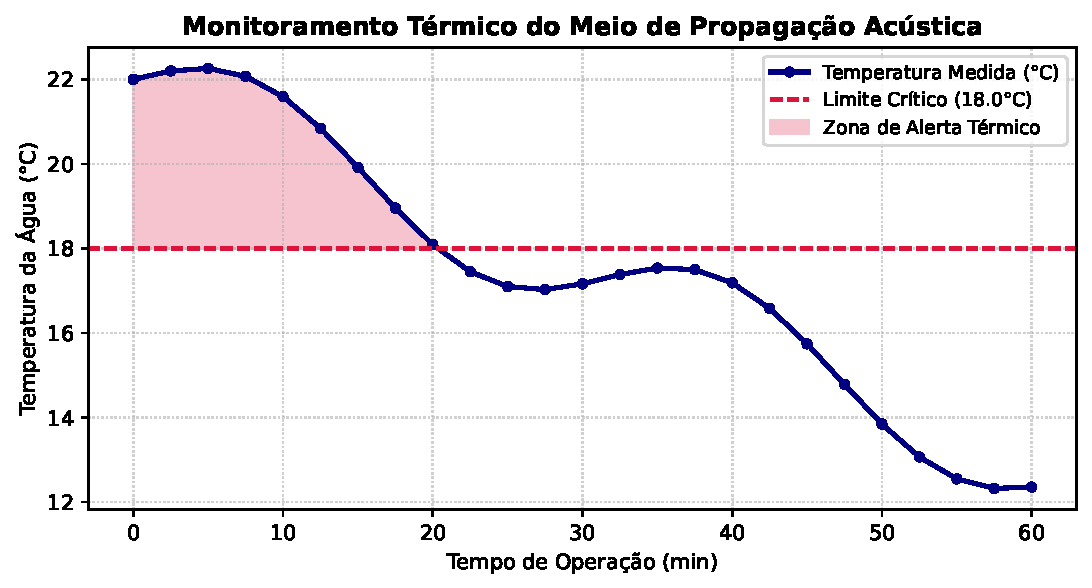
\includegraphics[width=0.88\linewidth]{body/Lista_12/figures/fig_Q9.pdf}
    \captionof{figure}{Saída gráfica gerada: curva temporal de temperatura com limiar crítico e zona de alerta sombreada.}
\end{center}
\fi
